%%%%%%%%%%%%%%%%%%%%%%%%%%%%%%%%%%%%%%%%%%%%%%%%%%%%%%%%%%%%%%%%%%%%%%
% LaTeX Example: Project Report
%
% Source: http://www.howtotex.com
%
% Feel free to distribute this example, but please keep the referral
% to howtotex.com
% Date: March 2011 
% 
%%%%%%%%%%%%%%%%%%%%%%%%%%%%%%%%%%%%%%%%%%%%%%%%%%%%%%%%%%%%%%%%%%%%%%
% How to use writeLaTeX: 
%
% You edit the source code here on the left, and the preview on the
% right shows you the result within a few seconds.
%
% Bookmark this page and share the URL with your co-authors. They can
% edit at the same time!
%
% You can upload figures, bibliographies, custom classes and
% styles using the files menu.
%
% If you're new to LaTeX, the wikibook is a great place to start:
% http://en.wikibooks.org/wiki/LaTeX
%
%%%%%%%%%%%%%%%%%%%%%%%%%%%%%%%%%%%%%%%%%%%%%%%%%%%%%%%%%%%%%%%%%%%%%%
% Edit the title below to update the display in My Documents
%\title{Project Report}
%
%%% Preamble
\documentclass[paper=a4, fontsize=11pt]{scrartcl}
\usepackage[T1]{fontenc}
\usepackage{fourier}

\usepackage[english]{babel}															% English language/hyphenation
\usepackage[protrusion=true,expansion=true]{microtype}	
\usepackage{amsmath,amsfonts,amsthm} % Math packages
\usepackage[pdftex]{graphicx}	
\usepackage{url}


%%% Custom sectioning
\usepackage{sectsty}
\allsectionsfont{\centering \normalfont\scshape}


%%% Custom headers/footers (fancyhdr package)
\usepackage{fancyhdr}
\pagestyle{fancyplain}
\fancyhead{}											% No page header
\fancyfoot[L]{}											% Empty 
\fancyfoot[C]{}											% Empty
\fancyfoot[R]{\thepage}									% Pagenumbering
\renewcommand{\headrulewidth}{0pt}			% Remove header underlines
\renewcommand{\footrulewidth}{0pt}				% Remove footer underlines
\setlength{\headheight}{13.6pt}


%%% Equation and float numbering
\numberwithin{equation}{section}		% Equationnumbering: section.eq#
\numberwithin{figure}{section}			% Figurenumbering: section.fig#
\numberwithin{table}{section}				% Tablenumbering: section.tab#


%%% Maketitle metadata
\newcommand{\horrule}[1]{\rule{\linewidth}{#1}} 	% Horizontal rule

\title{
		%\vspace{-1in} 	
		\usefont{OT1}{bch}{b}{n}
		\normalfont \normalsize \textsc{Artificial Intelligence} \\ [25pt]
		\horrule{0.5pt} \\[0.4cm]
		\huge Team-based Halma Artificial Intelligence\\
		\horrule{2pt} \\[0.5cm]
}
\author{
		\normalfont 								\normalsize
        Peter Henderson\\[-3pt]		\normalsize
        260457751\\ \normalsize
        \today
}
\date{}


%%% Begin document
\begin{document}
\maketitle
\section{Explanation of program and Motivation}

After attempting several techniques and running comparisons among the various players created (please see appropriate section for details), a modified depth limited search player was found to have the highest rate of winning and the fastest decision rate. The motivation behind using this technique (other than the fact that it outperformed all other players) was due to the AI's ability to choose complex hop sequences which would result in a winning board. An example of this can be seen in Figure 1. However, given a longer time period for thinking about moves (more than 1 second), perhaps the Monte Carlo player or the Mini-Max player developed would have been chosen. 
\begin{figure}[h!]
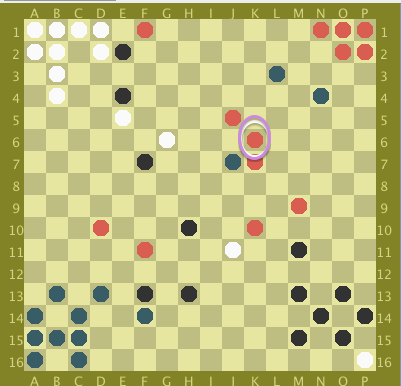
\includegraphics[scale=.2]{1}
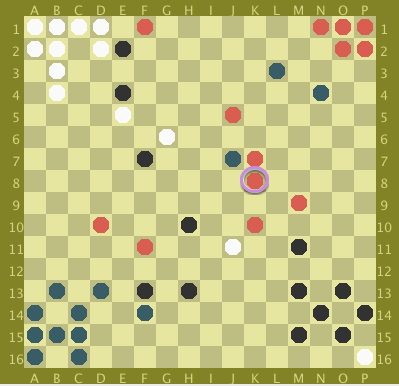
\includegraphics[scale=.2]{2}
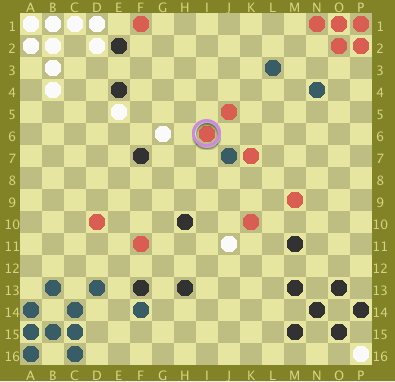
\includegraphics[scale=.2]{3}
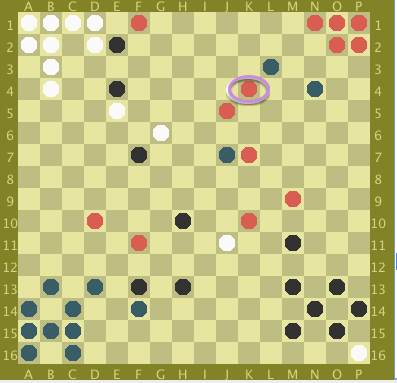
\includegraphics[scale=.2]{4}
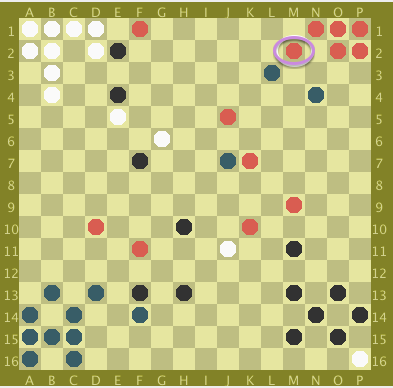
\includegraphics[scale=.2]{5}
\caption{A sequence of moves going backwards and around to find a better placement, highlighted with a purple circle.}
\end{figure}

\subsection{Heuristic}
The heuristic used for all players took into account domain knowledge to improve the performance of the players. For the base of the heuristic, the Manhattan distance to the goal base was subtracted from $32$ (the highest Manhattan distance possible) for each piece and added to the cumulative score. \\\\As incentive for keeping pieces in the base once they arrive, the number of pieces in the goal base multiplied by a constant factor is added to the score. To make sure that all pieces leave the home base as soon as possible to avoid losing the game, a weighted penalty is subtracted from the overall score for each piece in the home base. Lastly, a reward for staying closer to the diagonal between team bases is given to promote creating ``ladders'' between teams. At first another penalty was added for any piece which does not have another piece on its team in the surrounding area, but this proved to be detrimental to the winning rate and thus was removed.\\\\
To determine the best heuristic, each addition of reward/penalty/weight was tested by competing a player with the previous heuristic against the same player with the added penalty. If the new addition resulted in significant increases in winning rates, it was kept.

\subsection{The Final Algorithm}
The final algorithm used is essentially a modified greedy depth-limited search, where the limit is different between hops and normal moves. The algorithm iterates through each possible move of the first given board. If the move is a hop, it proceeds to a reasonable given depth to get the final state and evaluate this using the above heuristic. At each depth a comparison is made to the best score so far, so that if a certain depth is of greater score than later on in the sequence, the move ends there. Though there is functionality to go to a greater depth for non-hop moves, the large branching factor resulted in significant performance impacts and as such was not used for the final product. \\\\ The algorithm is greedy in that it takes the best next move with the greatest valued final board state. This obviously favors jumps as jumps are always extended to a greater depth for the evaluation state. 

\subsection{Pro/Cons}
This approach is extremely good at finding long jump sequences that place pieces in the goal state. This allows for moves that many other players would not find (such as best first search or certain implementations of Minimax and Monte Carlo search). Additionally, the heuristic used generally keeps pieces from straying too far from one another, resulting in fewer straggling pieces toward the end of the game. However, there are also several down sides to this approach. There are still some stragglers left. Though an attempt was made to add a weighted penalty for straying too far from a friendly piece in the heuristic, this underperformed when facing a similar player with a heuristic lacking this penalty and as such was omitted. Other attempts to keep pieces from falling behind also proved unsuccessful (mostly in modifying the heuristic). Additionally, the game player does not look for a ``real'' long term game plan. For example, it does not set up hop sequences purposefully, such as ladder sequences. By nature of the heuristic though, the pieces stay toward the diagonal so these ladder sequences happen by consequence of this without a ``real'' long-term game plan.

\section{Motivation and Previous Approaches}
\subsection{Motivation}
The motivation for the modified greedy depth-limited search approach was to find the best hop sequences, no matter which direction the player went on the first hop. For example, with a greedy best-first limited search, the player would not look at a backwards hop first, if at all, and as such could potentially miss a hop sequence that goes backwards but then wraps around to the goal state. The current version of the algorithm actually finds and chooses these moves. Additionally, the speed of this approach versus others in choosing a move greatly aided in making sure that the player did not reach the time limit.

\subsection{Previous Approaches}
In the $/previous$ directory of the source folder there are several other players that were developed and tested against one another to try and find the best one. The first player that was developed was a player that utilized Alpha-Beta pruning to try to find the best move. At first the heuristic was modified such that it took all players into account (such that an opponents move would actually lower the given players score for the min layer). However, the large branching factor of Minimax resulted in a maximum depth of 4 (i.e. only the next turn of the current player) which took several seconds to compute. Even then, the result was not always favorable. After trying to decrease the branching factor through added pruning (opponent's moves were chosen at random toward the beginning/end of the game as they don't affect the player), the results were still too slow for the given time limit for any significant depth. \\\\After this the previously described greedy player was created which preformed well. Then the greedy player was modified with a pseudo-Monte Carlo rollout stage for each move adding to the weight of the score. So for each move, the heuristic score was found. Then several random games were played until a certain depth and the final average of all the random games from that state was weighted and added to the heuristic score. This actually decreased the performance of the greedy player in most scenarios (though in one trial it did in fact beat the greedy player, but this could not be recreated due to the random nature of the rollout). \\\\A ``real'' Monte Carlo search player was then attempted. A Monte Carlo search tree was kept in memory and ran through the 4 phases of Monte Carlo search (Descent, Rollout, Update, Growth). When choosing a move, the previous nodes were nullified for clean up by the Garbage Collector and when the players chose their turns, the current node was updated to match the real state of the board. In this way some of the next states could be precomputed. Though this worked fairly well for a lower number of iterations (around 100), it still did not beat the greedy player. A higher number of iterations resulted in heap overflows because the garbage collector could not keep up. 

\section{Improvements}
Part of the reason many of the other approaches wouldn't work as well (and why the current player did not see very far into the future), was due to the time limitations for choosing a move. Perhaps by lowering down the amount of memory that a board takes up, or creating a smaller representation of a board for Monte Carlo, larger amounts of rollouts could have worked. Or by excessively pruning the second layer of moves, the given player could have gone to much greater depth for non-hop moves also to try and setup smarter hop sequences later on. Though this pruning was attempted, it did not benefit the player in any significant way. Perhaps a better approach overall would have been to optimize all code to the bit level to make a much more efficient approaching to handling so many branches. In this way, Monte Carlo or Minimax may have outperformed the greedy player.
\\\\
With optimizations for the Board representation or added pruning perhaps the Greedy player could have gone to a much greater depth, resulting in a winning strategy. However, due to the nature of the Project setup and time constraints (the CCBoard object, etc.), these optimizations were not attempted. Perhaps by storing just a move for Monte Carlo rather than a board and ranking a CCMove rather than a whole CCBoard with the heuristic, the time and space complexity could have gone down. However, this would leave only a limited view of the playing field and would decrease the effectiveness of the heuristic.

%%% End document
\end{document}